\documentclass{article}

\usepackage{graphicx}
\usepackage{csvsimple}
\usepackage[numbers]{natbib}
\usepackage[affil-it]{authblk}

\bibliographystyle{apalike}

\begin{document}
\title{A Multi-Scale Analysis of 27,000 Urban Street Networks\footnote{This is a journal article manuscript currently under peer review.}}
\author{Geoff Boeing\footnote{Email address: gboeing@berkeley.edu; corresponding author.}}
\affil{Department of City and Regional Planning\\University of California, Berkeley}
\date{\today}
\maketitle

\begin{abstract}
OpenStreetMap presents an emerging source of worldwide geospatial urban data useful to researchers. This paper uses the OSMnx software to automatically download and analyze 27,000 street networks from OpenStreetMap at metropolitan, municipal, and neighborhood scales---that is, every urbanized area, incorporated place, and Zillow neighborhood in the US. In turn it presents wide-ranging empirical findings on US urban form and street network characteristics. This paper addresses past limitations by conducting an analysis of street networks with an extremely large sample sizes, with clearly defined network definitions and extents for reproducibility, and using non-planar, directed graphs. Its analysis emphasizes urban street networks measures relevant to urban design and morphology, including structure, connectedness, centrality, and robustness. In total we cross-sectionally analyze the street networks of 497 urbanized areas, 19,655 cities and towns, and 6,857 neighborhoods. These sample sizes are larger than those in any previous study and illustrate the use of OSMnx and OpenStreetMap as a new urban form research platform.
\end{abstract}

\section{Introduction}
On May 20, 1862, Abraham Lincoln signed the Homestead Act into law, making land across the United States Midwest and Great Plains available for free to all applicants \cite{porterfield_homestead_2005}. Under its auspices over the next 70 years, the federal government distributed 270 million acres of public land (10\% of the entire US landmass) to private owners in the form of 1.6 million homesteads \cite{lee_kansas_1979, sherraden_inclusion_2005}. Towns with gridiron street networks sprang up rapidly across the Great Plains and Midwest, due to both the prevailing urban design paradigm of the day and the standardized rectilinear town plats used repeatedly to lay out instant new cities \cite{southworth_streets_1997}. Through path dependence, the spatial signatures of these land use laws, design paradigms, and planning instruments can still be seen today in these cities' urban forms and street networks.

A cross-sectional analysis of American urban form through its street networks at metropolitan, municipal, and neighborhood scales can reveal these artifacts and histories across the nation. Network analysis is a natural approach to the study of cities as growing, complex systems that self-organize to fill space with a capillary circulation network \cite{masucci_random_2009}. The empirical literature on street network analysis is growing ever richer, but suffers from some limitations---discussed in \cite{boeing_osmnx:_2017} and summarized here. First, sample sizes tend to be fairly small due to data availability, gathering, and processing constraints. Second, reproducibility is difficult when the dozens of decisions that go into analysis---such as spatial extents, topological simplification and correction, definitions of nodes and edges, etc.---are ad hoc or only partly reported. Third, and related to the first two, studies frequently oversimplify to planar or undirected primal graphs for tractability, or use dual graphs despite the loss of geographic and metric information. 

This paper addresses these limitations by conducting an analysis of street networks at multiple scales, with large sample sizes, with clearly defined network definitions and extents for reproducibility, and using non-planar, directed graphs. In particular, it examines urban street networks---represented here as primal, non-planar, weighted multidigraphs with possible self-loops---focusing on structure, connectedness, centrality, and resilience. Most studies in the street network literature that conduct topological and/or metric analysis tend to have sample sizes ranging around 5 to 50 networks. This paper instead conducts a large analysis of over 27,000 urban street networks at multiple overlapping scales across the United States. Namely, it examines the street networks of every US incorporated city and town, urbanized area, and Zillow-defined neighborhood. In total, this study presented uses OSMnx \cite{boeing_osmnx:_2017} to download, construct, and analyze 497 urbanized areas' street networks, 19,655 cities' and towns' street networks, and 6,857 neighborhoods' street networks. It uses these street networks to conduct four analyses: at the metropolitan scale, at the municipal scale, at the neighborhood scale, and with a case study looking deeper at the neighborhood-scale street networks in the city of San Francisco.

This paper is organized as follows. In the next section, it presents the data sources, tools, and methods used to collect, construct, and analyze these street networks. Then it presents findings of the analyses at three spatial scales: metropolitan, municipal, and neighborhood. Finally, it concludes with a discussion of these findings and their implications for street network analysis, urban form complexity, and city planning.

\section{Methodology}
This study uses OSMnx to download, construct, correct, analyze, and visualize street networks at metropolitan, municipal, and neighborhood scales \cite{boeing_osmnx:_2017}. To define the study sites and their spatial boundaries, this study uses three sets of geometries. The first defines the metropolitan-scale study sites using the 2016 national TIGER/Line shapefile of US census bureau urban areas, released 19 August 2016. Census-defined urban areas comprise a set of census tracts that meet a minimum density threshold \cite{u.s._census_bureau_2010_2010}. In particular, we retain only the urbanized areas subset in this data set (i.e., areas with greater than 50,000 population), discarding the smaller urban clusters subset. The second set of geometries defines the municipal-scale study sites using 51 TIGER/Line shapefiles (again, 2016) of US census bureau places for all 50 states plus the District of Columbia. In particular, we discard the subset of census-designated places in this data set, instead retaining all the incorporated cities and towns in the United States. 

The third and final set of geometries defines the neighborhood-scale study sites using 42 Zillow neighborhood shapefiles. These shapefiles contain the geometries of neighborhoods in 41 states plus the District of Columbia. This is a fairly new data set comprising nearly 7,000 neighborhoods in large American cities, but as \citet{schernthanner_spatial_2016} point out, Zillow does not publish the methodology it uses to construct these geometries. However, despite its newness it already has a track record in the academic literature. For instance, \citet{besbris_effect_2015} used Zillow boundaries to examine neighborhood stigma, and \citet{albrecht_indicator_2014} used these data to study neighborhood-level poverty in New York.

For all of these geometries, we use OSMnx to download the (drivable, public) street network contained within the geometry. First it buffers each geometry by 0.5 km, then downloads the street network within this buffered geometry. Next it constructs a street network from this data, corrects the topology, calculates street counts per node (this ensures that intersections are not considered cul-de-sacs simply because an incident edge connects to a node outside the desired polygon), then truncates the network to the original, desired polygon. OSMnx saves each of these networks to disk as GraphML and shapefiles. Finally, it automatically calculates metric and topological measures for each. However, in a planar graph, topological and metric properties are somewhat interrelated \cite{masucci_random_2009}.

Average street length, the mean edge length in the undirected representation of the graph, serves as a linear proxy for block size and indicates how fine-grained or coarse-grained the network is. Node density is the number of nodes divided by the area covered by the network. Intersection density is the node density of the set of nodes with more than one street emanating from them (thus excluding dead-ends). The edge density is the sum of all edge lengths divided by the area, and the physical street density is the sum of all edges in the undirected representation of the graph divided by the area. These density measures all provide further indication of how fine-grained the network is. Finally, the average circuity represents the average ratio between an edge length and the straight-line distance between the two nodes it links.

The average node degree, or mean number of edges incident to each node, quantifies how well the nodes are connected on average. Similarly, but more concretely, the average streets per node measures the mean number of physical streets (i.e., edges in the undirected representation of the graph) that emanate from each intersection and dead-end. This adapts the average node degree for physical form rather than directed circulation. The statistical and spatial distributions of number of streets per intersection characterize the type, prevalence, and dispersion of intersection connectedness in the network. Connectivity measures the minimum number of nodes or edges that must be removed from a connected graph to disconnect it. The average node connectivity of a network---the mean number of internally node-disjoint paths between each pair of nodes in the graph---represents the expected number of nodes that must be removed to disconnect a randomly selected pair of non-adjacent nodes \cite{beineke_average_2002}. 

The clustering coefficient of a node is the ratio of the number of edges between its neighbors to the maximum possible number of edges that could exist between these neighbors. The weighted clustering coefficient weights this ratio by edge length and the average clustering coefficient is the mean of the clustering coefficients of all the nodes in the network. Centrality indicates the importance of nodes in a network. Betweenness centrality evaluates the number of shortest paths that pass through each node \cite{barthelemy_betweenness_2004}. The maximum betweenness centrality in a network specifies the proportion of shortest paths that pass through the most important node. This is an indicator of resilience: networks with a high maximum betweenness centrality are more prone to failure or inefficiency should this single choke point fail. Closeness centrality ranks nodes as more central if they are on average closer to all other nodes. Finally, PageRank ranks nodes based on the structure of incoming links and the rank of the source node.

In total, this study cross-sectionally analyzes 27,009 networks: 497 urbanized areas' street networks, 19,655 cities' and towns' street networks, and 6,857 neighborhoods' street networks. These sample sizes are larger than those in any previous study. In the following sections, we present the findings of these analyses at the metropolitan scale, the municipal scale, the neighborhood scale, and through a case study looking deeper at the neighborhood-scale street networks in the city of San Francisco.

\section{Analysis of Metropolitan-Scale Street Networks}

\begin{table*}[hp]
\caption{Central tendency and statistical dispersion for selected measures of all US urbanized areas' street networks.}
\label{table01}
\csvautotabular{media/table01.csv}
\end{table*}

Table \ref{table01} shows the considerable variation in street network characteristics across the entire data set of 497 urbanized areas. This is unsurprising: urbanized areas span a wide spectrum of sizes, from the Delano, CA Urbanized Area's 26 km\textsuperscript{2} to the New York--Newark, NY--NJ--CT Urbanized Area's 8,937 km\textsuperscript{2}---thus, density and count-based measures demonstrate substantial variance. Further, these urbanized areas span a wide spectrum of terrains, development eras and paradigms, and cultures.

\begin{figure*}[h]
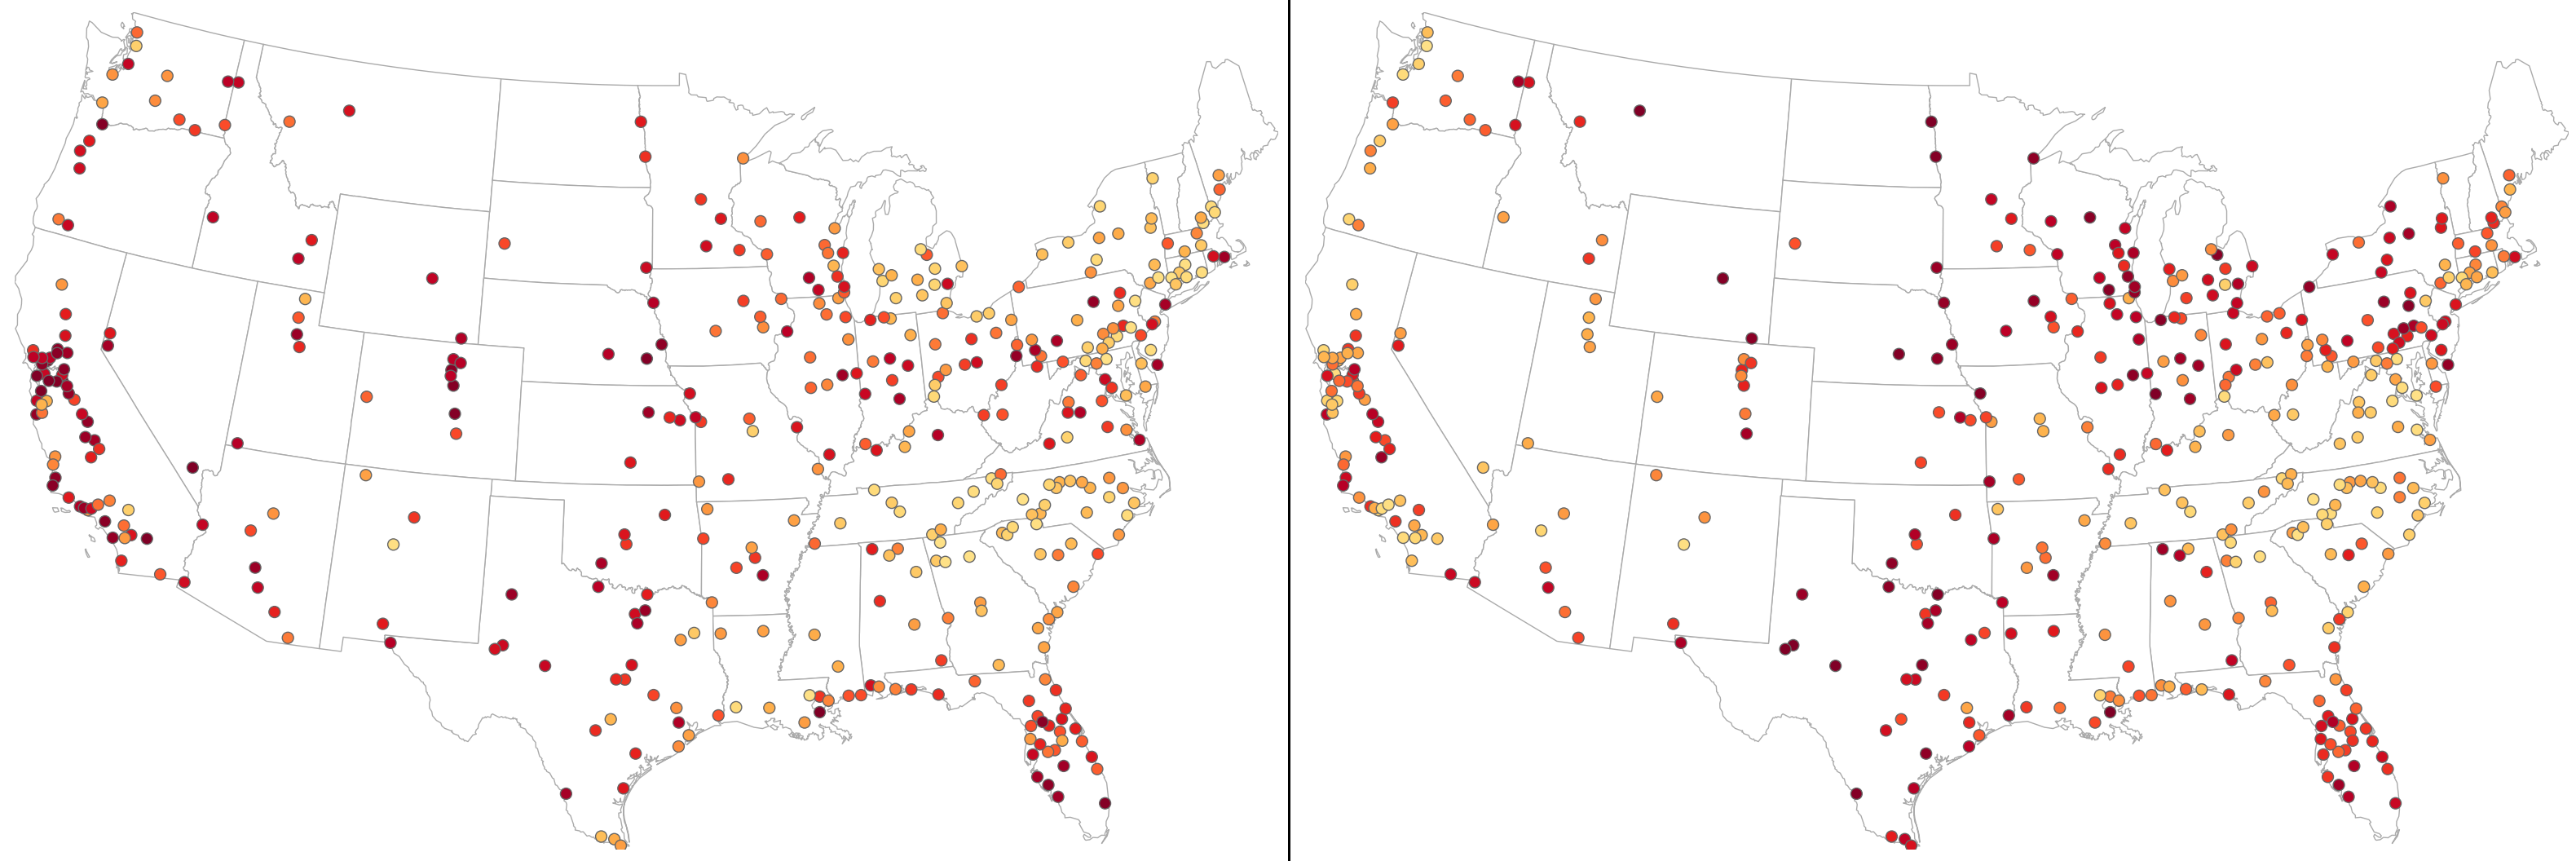
\includegraphics[width=1\textwidth]{media/fig01.png}
\caption{Intersection density per urbanized area (left) and average streets per node per urbanized area (right) from lowest (pale yellow) to highest (dark red), in the contiguous US}
\label{fig01}
\end{figure*}

Nevertheless, looking across the data set provides a sense of the breadth of American metropolitan street networks. New York's urbanized area---America's largest-–-has 373,309 intersections and 79 million meters of linear street (or 417,570 and 83.4 million if including service roads). Delano, CA's urbanized area---America's smallest---has 874 intersections and 222,328 meters of linear street (or 964 and 231,000 meters if including service roads). The typical (Table \ref{table01}, \emph{median}) American urbanized area is approximately 185 km\textsuperscript{2} in land area, has 5,830 intersections, and 1.3 million linear meters of street. Its street network is about 7.4\% more circuitous than straight-line, as-the-crow-flies edges between nodes would be. The most circuitous network is 14\% more circuitous than straight-line would be, and least is only 2\%. Looking at network complexity in terms of density and connectivity, in the typical urbanized area, the average street segment length (a proxy for block size) is 160 meters. The longest average street segment is the 226-meter average of urbanized Danbury, CT. Puerto Rican cities hold the top four positions for shortest average street segment length, but among the 50 states plus DC, the shortest average street segment is the 125.3-meter average of urbanized Tracy, CA, indicating a much finer street network. The urbanized area of Portland, Oregon, with its famously compact walkable blocks, ranks second at 125.5 meters on average.

\begin{figure*}[hp]
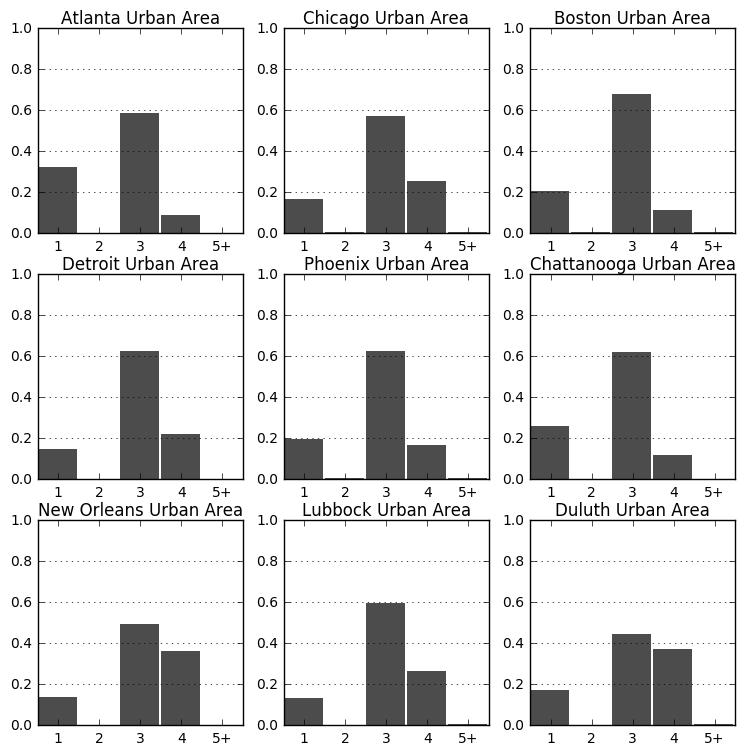
\includegraphics[width=1\textwidth]{media/fig02.png}
\caption{Distribution of node types in 9 urbanized areas, with number of streets emanating from the node on the $x$-axis and proportion of nodes of this type on the $y$-axis }
\label{fig02}
\end{figure*}

The typical urbanized area has 26 intersections per km\textsuperscript{2}. Both the densest and the sparsest are in the deep south: the sparsest is 12.5 (Gainesville, GA urbanized area) and the densest is 49.4 (New Orleans urbanized area). However, New Orleans is an anomaly in the deep south. Figure \ref{fig01} depicts the intersection density in each American urbanized area, from lowest density in dark red to highest density in light yellow. The map makes clear how the highest intersection densities are concentrated to the west of the Mississippi River. The lowest intersection densities are concentrated in a belt running from Louisiana, up through the Carolinas and Appalachians, and into New England. In general, only the largest cities on the east coast (e.g., Boston, New York, Philadelphia, Washington) and Florida escape this trend.

The distribution of node types (i.e., intersections and dead ends) provides a clear indicator of network connectedness. The typical urbanized area has 2.8 streets per intersection on average: lots of 3-way intersections, fewer cul-de-sacs, and even fewer 4-way intersections. The grid-like San Angelo, TX urbanized area has the most streets per node (3.2) on average, and (outside of Puerto Rico, which contains the seven lowest urbanized areas) the sprawling, disconnected Lexington Park, MD urbanized area has the fewest (2.2). These two urban areas fit the trend seen in the spatial distribution across the US in Figure \ref{fig01}: urbanized areas in the great plains and Midwest have particularly high numbers of streets per node on average, indicating more grid-like, connected networks. Cities in the southern and western US tend to have fewer streets per node, reflecting more dead-ends and a disconnected network. This finding is discussed in more detail in the upcoming section.

In the typical urbanized area, 18\% of nodes are 4-way intersections, 59\% are 3-way intersections, and 21\% are dead-ends. However, this distribution varies somewhat between urbanized areas. Examining a small sample of 9 urbanized areas, chosen to maximize variance, reveals this in clearer detail. In Figure \ref{fig02}, urban Atlanta and Chattanooga have very high proportions of dead-ends, each over 30\% of all nodes, and very few 4-way intersections, indicating a disconnected street pattern. The urban areas of Phoenix, Boston, Detroit, and Chattanooga have particularly high proportions of 3-way intersections, each over 60\%, indicating a prevalence of T-intersections. Conversely, Chicago, New Orleans, Duluth, and Lubbock have high proportions of 4-way intersections, indicating more grid-like connected networks. But what is perhaps most notable about Figure \ref{fig02} is that these nine urbanized areas, despite being chosen to maximize variance, are overwhelmingly similar to each other. At the metropolitan scale, every large American urban agglomeration is characterized by a preponderance of 3-way intersections.

The relationship between fine-grained networks and connectedness/grid-ness is, however, not clear-cut. Intersection density has only a weak, positive linear relationship with the proportion of 4-way intersections in the urbanized area ($r^{2}=0.17$). But the relationship between network circuity and grid-ness is somewhat clearer. Average circuity has a negative linear relationship with the proportion of 4-way intersections in the urbanized area ($r^{2}=0.43$).

\begin{table*}[hp]
\caption{Selected measures of the 30 largest (by land area) urbanized areas' street networks.}
\label{table02}
\csvautotabular{media/table02.csv}
\end{table*}

Due to the substantial variation in urbanized area size, from 25 to 9,000 km\textsuperscript{2}, the preceding analysis covers a wide swath of metropolitan place types. To better compare apples-to-apples, Table \ref{table02} focuses on the 30 largest urban areas cross-sectionally to examine how their metric and topological measures compare. This provides more consistent spatial scales and extents, while offering a window into the similarities and differences in the built forms of America's largest urban agglomerations. 

Among these urban areas, Milwaukee has the least circuitous network (6\% more circuitous than straight-line edges would be), and Orlando has the most (12\%). San Juan and Atlanta have the fewest streets per node on average (2.36 and 2.45, respectively), while Milwaukee has the most (3.03). Cincinnati has both the lowest intersection density (18/km\textsuperscript{2}) and street density (6.1 km/km\textsuperscript{2}) while Denver has the highest intersection density (40.6/km\textsuperscript{2}) and Miami and Los Angeles have the highest street density (10.6 km/km\textsuperscript{2}, apiece). In other words, Cincinnati has a particularly coarse-grained network with few connections and paths. This can also be seen in the average street segment length, a proxy for block size: Cincinnati has the second highest (186 m), bested only by Cleveland (198 m). In contrast, the two lowest are Denver's 138-meter average and San Juan's 131-meter average.

These metropolitan-scale analyses consider trends in the built form at the scale of broad self-organized human systems and urbanized regions. However, they aggregate multiple heterogenous neighborhoods and municipalities---the scales of human life, urban design projects, and planning jurisdiction---into single units of analysis. To disaggregate and analyze finer characteristics, the following sections examine municipal- and neighborhood-scale street networks across the United States.

\section{Analysis of Municipal-Scale Street Networks}

Table \ref{table03} shows similarly great variation in street network characteristics across the entire data set of 19,655 cities and towns. Again, this data set comprises the street networks of every incorporated city and town in the United States. Following recent work by \citet{barthelemy_modeling_2008} and \citet{strano_urban_2013}, we examine the relationship between the total street length $L$ and the number of nodes $n$. The former proposed a model of cities in which $L$ and $n$ scale nonlinearly as $n^{1/2}$, and the latter recently confirmed this empirically with a small sample of ten European cities' street networks. However, their small sample size may limit the generalizability and interpretability of their finding. To investigate this empirically, we examine the relationship between the total street length $L$ and the number of nodes $n$ for 19,655 US cities and towns and find a strong \emph{linear} relationship ($r^{2}=0.98$), as depicted in Figure \ref{fig03}, contradicting Strano et al. We also find a similar linear relationship at the metropolitan and neighborhood scales.

\begin{table*}[hp]
\caption{Selected summary stats for every incorporated city and town in the US.}
\label{table03}
\csvautotabular{media/table03.csv}
\end{table*}

\begin{figure*}[h]
	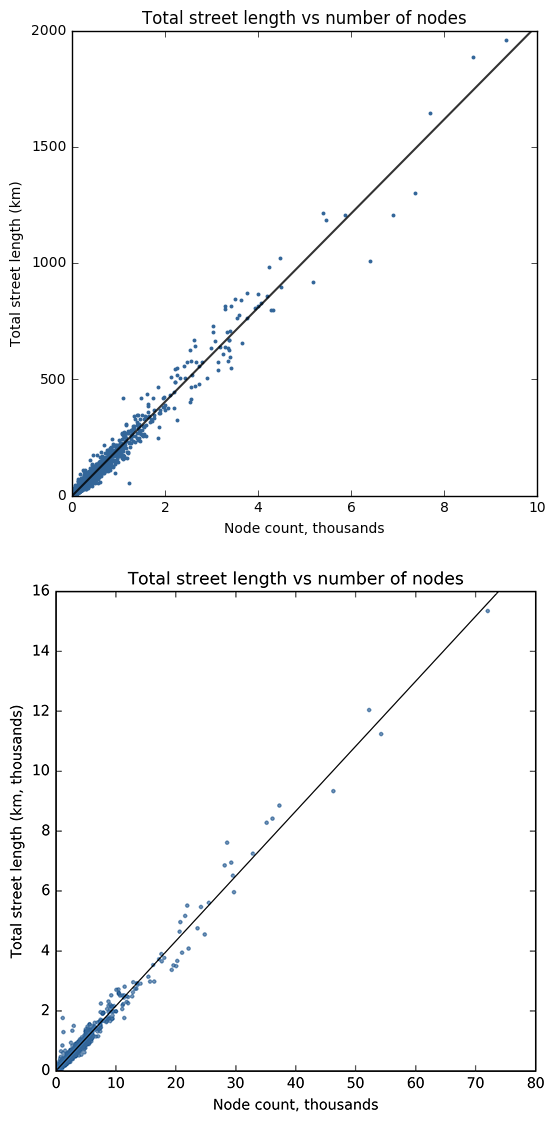
\includegraphics[width=1\textwidth]{media/fig03.png}
	\caption{The linear relationship between total street length and number of nodes in the street networks of 6,857 US neighborhoods (top) and 19,655 US cities and towns (bottom).}
	\label{fig03}
\end{figure*}

\begin{figure*}[h]
	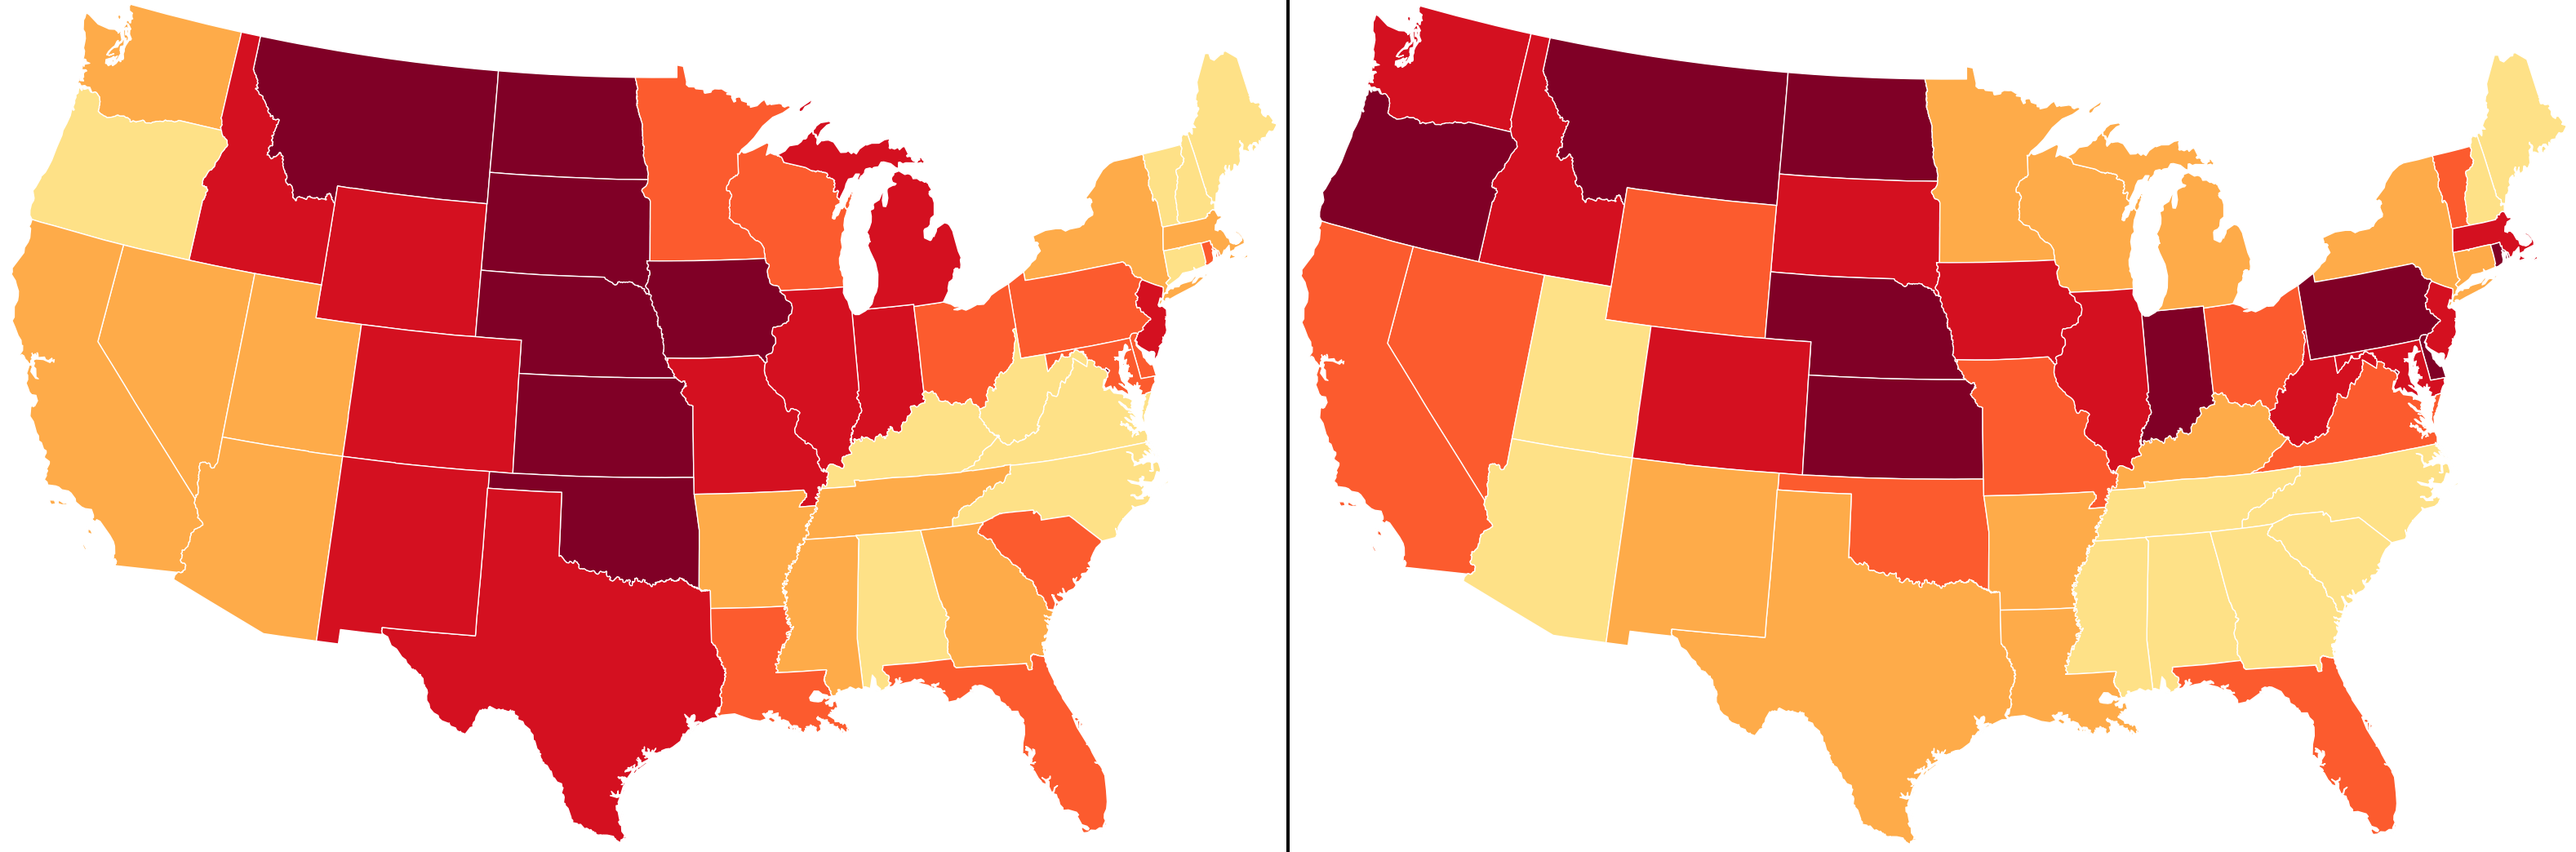
\includegraphics[width=1\textwidth]{media/fig04.png}
	\caption{Left: contiguous US states by median of mean streets per node in municipal street networks, from lowest (pale yellow) to highest (dark red). Right: contiguous US states by median of mean street segment length in municipal street networks, from longest (pale yellow) to shortest (dark red).}
	\label{fig04}
\end{figure*}

Moreover, previous findings \citep[e.g.,][]{masucci_random_2009} suggest the distribution of street segment lengths in an urban street network follows a power-law distribution. However, we find that these networks instead generally follow a lognormal distribution, which makes theoretical sense as most street networks are not truly scale-free. For example, a typical street network might comprise very few very long street segments (e.g., 1 km), more medium-length segments (e.g., 250 m), and many short segments (e.g., 80 m), but very few very short segments (e.g., 10 m). This theoretical illustration suggests the lognormal distribution that this study generally finds across municipal US street networks. An exception, of course, lies in consistently-sized orthogonal grids filling a city's incorporated spatial extents. Such distributions are extremely peaked around a single value: the linear length of a grid block.

This study finds that such cities are not uncommon, particularly between the Mississippi River and the Rocky Mountains: the Great Plains states are characterized by a unique street network form that is both orthogonal and reasonably dense. The former is partly the result of topography (flat, plains terrain that allows idealized grids) and design history (platting and development during the late nineteenth century) that favor orthogonal grids, as discussed earlier. The latter results from the fact that most towns across the Great Plains exhibit minimal suburban sprawl. Thus, the municipal boundaries snugly embrace the grid-like street network, without extending to accommodate the vast peripheral belt of twentieth century sprawl, circuity, and ``loops and lollipops" \cite{southworth_streets_1997} that characterizes cities in California that were settled in the same era but later subjected to substantial suburbanization.

\begin{table*}[hp]
\caption{Median values, aggregated by state plus DC, of selected measures of the municipal-scale street networks for every city and town in the US.}
\label{table04}
\csvautotabular{media/table04.csv}
\end{table*}

For example, if we measure connectedness in terms of average number of streets per node at the city-scale and then aggregate these cities by state (Table \ref{table04}), we find Nebraska, Kansas, South Dakota, Montana, North Dakota, Oklahoma, and Iowa have, in order, the highest medians (Figure \ref{fig04}). This indicates the most grid-like networks. If we measure density and connectedness in terms of intersection density---previously identified as an emergent property of complex network organization---at the city-scale and then aggregate these cities by state, we find Rhode Island, Nebraska, New Jersey, Kansas, and Montana have, in order, the highest medians. We again see three Great Plains states near the top, alongside densely populated East Coast states. Nebraska also has the smallest block sizes (measured via the proxy of average street segment length) while the largest are concentrated in the deep South, upper New England, and Utah (Figure \ref{fig04}).

Municipal boundaries vary greatly in their extents around the built-up area. For example, while Rhode Island averages 56 intersections/km\textsuperscript{2} in its cities and towns, Alaska averages only 1.3. This is an artifact of Alaska's municipal boundaries often extending thousands of square kilometers beyond the actual built-up area. In fact, Alaska has four cities (Anchorage, Juneau, Sitka, and Wrangell) with such large municipal extents that their land areas exceed that of the state of Rhode Island. These state-level aggregations of municipal-scale street network characteristics show clear variation across the country that reflect topography, economies, culture, planning paradigms, and settlement eras. But they also aggregate and thus obfuscate the variation within each state and within each city. To explore these smaller-scale differences, the following section examines street networks at the neighborhood scale.

\section{Analysis of Neighborhood-Scale Street Networks}

Thus far, we have examined every urban street network in the United States at the metropolitan and municipal scales. This analysis has focused on the complexity on the network in terms of density, resilience, and connectedness. While the metropolitan scale captures the emergent character of the wider region's complex system, and the municipal scale captures planning decisions made by a single city government, the neighborhood scale best represents the scale of individual urban design interventions into the urban form. Further, this scale more commonly reflects individual designs, eras, and paradigms in street network development than the ``many hands, many eras" evolution of form at larger scales.

\begin{table*}[hp]
\caption{Selected summary stats for all the neighborhood-scale street networks.}
\label{table05}
\csvautotabular{media/table05.csv}
\end{table*}

Table \ref{table05} presents summary statistics for this data set. Compared to the summary statistics presented at the metropolitan scale (Table \ref{table01}) and the municipal scale (Table \ref{table03}), here we see much greater variance. This is expected, given the smaller network sizes at the neighborhood scale. A few neighborhoods have no intersections within their Zillow-defined boundaries, resulting in a minimum intersection density of 0 across the data set. Meanwhile, the small neighborhood of Cottages North in Davis, California has the highest intersection density in the country, 444/km\textsuperscript{2}, largely as an artifact of its small area as the denominator. 

Nationwide, the typical neighborhood averages 2.9 streets per intersection, reflecting the prevalence of 3-way intersections in the US, discussed earlier. The median proportions of each node type are 14.5\% for cul-de-sacs, 57.4\% for 3-way intersections, and 23.4\% for 4-way intersections. The typical neighborhood averages 135-meter street segment lengths and 46.4 intersections per km\textsuperscript{2}. At the neighborhood scale (sample size of 6,857 in this analysis) we again find the same strong \emph{linear} relationship between total street length and the number of nodes in a network ($r^{2}=0.98$), as seen in Figure \ref{fig03}, contradicting the smaller-sample findings of \citet{strano_urban_2013}.

Due to the extreme values seen---resulting from the large variance in neighborhood size---we can filter the data set to examine only large neighborhoods (i.e., with area greater than the median value across the data set). In this filtered set, the five neighborhoods with the highest intersection density are all in central Philadelphia. Central neighborhoods are common at the top of this list, including Point Breeze, Philadelphia; Central Boston; Central City, New Orleans; Downtown Tampa; and Downtown Portland (Figure \ref{fig05}). The three neighborhoods with the lowest intersection density are on the outskirts of Anchorage, Alaska. In this filtered set, the neighborhoods with the greatest average number of streets per node tend to be older neighborhoods with orthogonal grids, such as Virginia Park, Tampa; Outer Sunset, San Francisco; and New Orleans' French Quarter. The neighborhoods with the lowest tend to be sprawling and often hilly suburbs far from the urban core, such as Scholl Canyon in Glendale, California or Sonoma Ranch in San Antonio, Texas.

\begin{figure*}[h]
	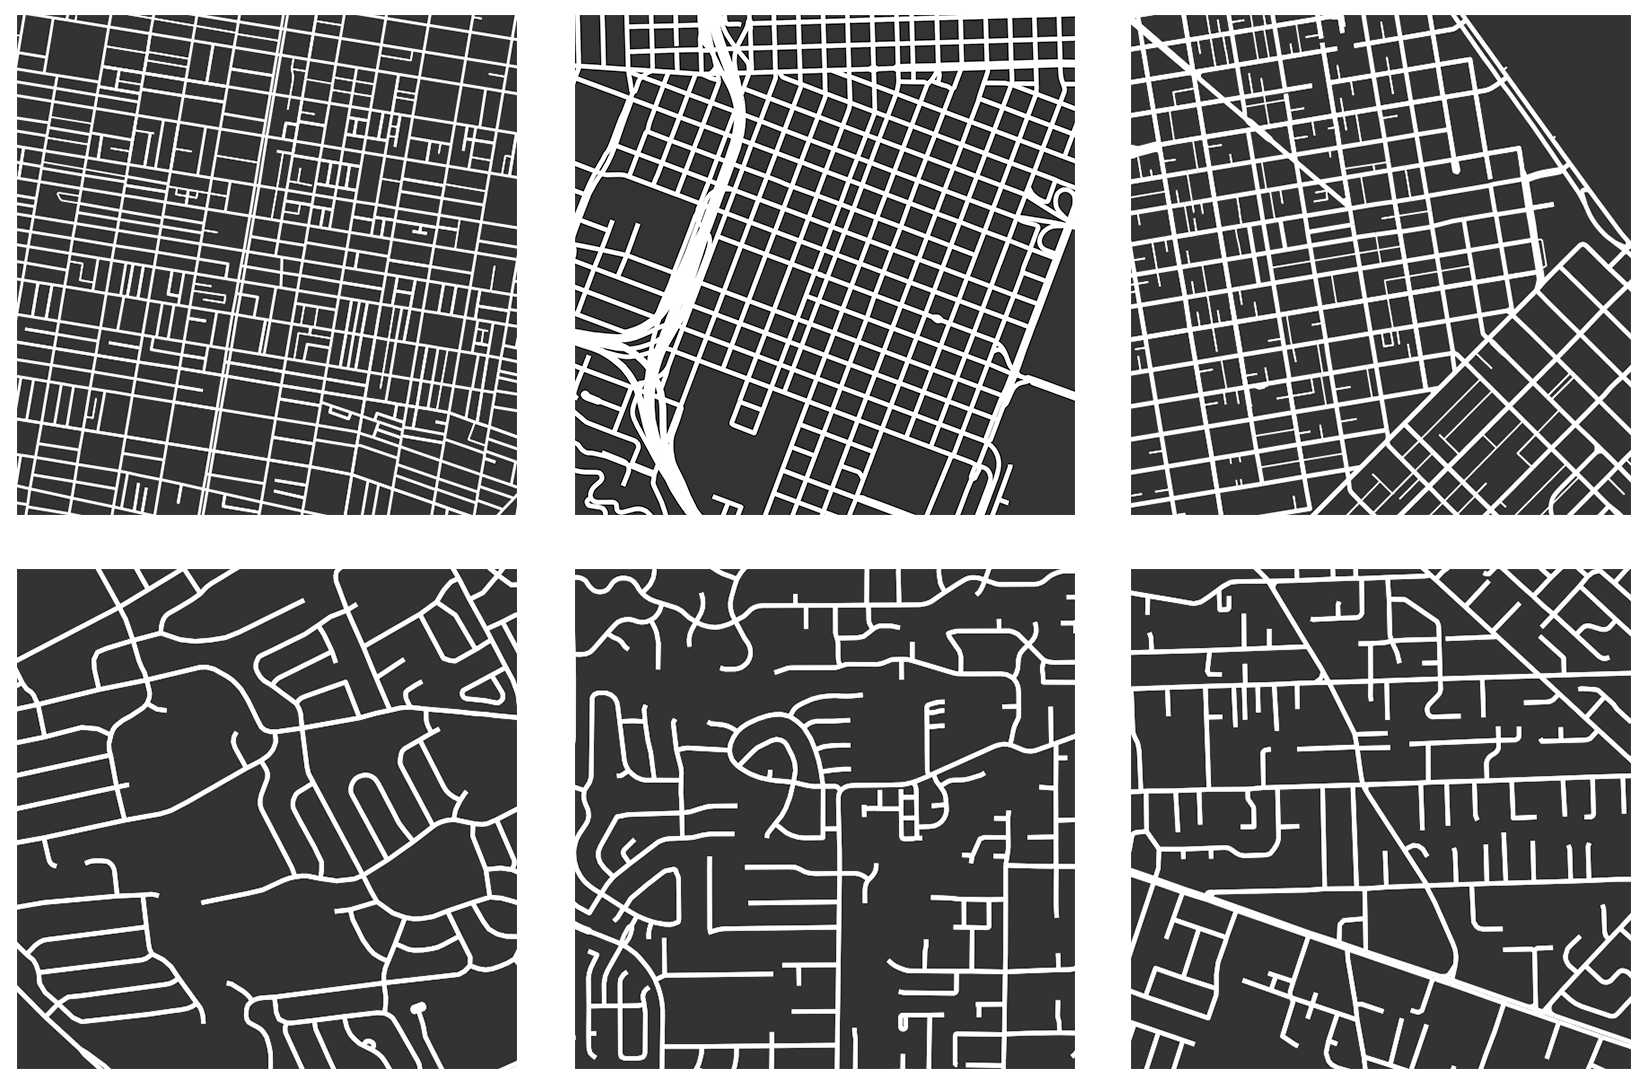
\includegraphics[width=1\textwidth]{media/fig05.png}
	\caption{Square-mile comparisons of central cities and their suburbs. Left: top, downtown Philadelphia; bottom, its suburb, King of Prussia. Middle: top, downtown Portland; bottom, its suburb, Beaverton. Right: top, downtown San Francisco; bottom, its suburb, Concord.}
	\label{fig05}
\end{figure*}

For comparison, Figure \ref{fig05} compares one square mile of the centers of Philadelphia, Portland, and San Francisco with one square mile of each of their suburbs. The connectedness and density of the central cities is clear, as is the disconnectivity of their suburbs. In fact, the suburbs have more in common with one another---despite being hundreds or thousands of miles apart---than they do with their central city neighbors, suggesting that land use and an era's prevailing design paradigm is paramount to geographical localism and regional context. The top row of Figure \ref{fig05} represents an era of urban planning and development that preceded the automobile, while the bottom row reflects the exclusionary zoning and mid-late twentieth century era of automobility in residential suburb design---namely the ``loops and lollipops" and the ``lollipops on a stick" design patterns identified by \citet{southworth_streets_1997}.

\section{Discussion}

A complex spatial network is a network, embedded in space, that has a nontrivial topology. In other words, its structure and organization is neither fully regular nor fully random. Of the network measures, this empirical study has presented preliminary findings that emphasize street network complexity in terms of density, resilience, and connectedness. Older, denser, and more self-organized networks, such as those at the heart of Boston or lower Manhattan are complex in terms of category I complexity. Sprawling, disconnected suburban neighborhoods rank low on all measures of complexity, with the exception that their high circuity can lend itself to disorder (i.e., category I). The orthogonal grid we see in the downtowns of Portland and San Francisco have high density (i.e., intersection and street densities), connectedness (i.e., average number of streets per node), and order (based on circuity and statistical dispersion of node types), but low resilience in the presence of one-way streets, measured by maximum betweenness centralities and average node connectivity increases when switching from one-way to bi-directional edges. These latter neighborhoods are complex in terms of category II and category III complexity. Their connectedness, density, and orderliness balances at the midpoint embraced by category II. However, their extreme regularity of block sizes, streets per node, and orthogonality best represents category III.

Another critical takeaway of this analysis is that scale matters. The median average circuity is lower across the neighborhoods data set than across the municipal set, which in turn is lower than across the urbanized areas set. Conversely, the median average number of streets per node is higher across the neighborhoods data set than across the municipal set, which in turn is higher than across the urbanized areas set. The median intersection density per km\textsuperscript{2} is about 83\% higher in the neighborhoods data set than in the municipal or urbanized areas sets. These findings make sense: the Zillow neighborhood boundaries focus on large, core cities with older and denser street networks. The municipal boundaries only include incorporated cities and towns---discarding small census-designated places and unincorporated communities. The urbanized area boundaries include far-flung sprawling suburbs.

The characteristics of an urban network for a city fundamentally depend on what city means: municipal boundaries, urbanized areas, or just certain neighborhoods? The first is a merely legal definition, but also captures the scope of city planning authority and decision-making for top-down interventions into a street network. The second captures a wider self-organized human system and its emergent built form, but tends to aggregate multiple non-homogenous built forms together into a single unit of analysis. The third captures the nature of the local built form and lived experience, but at the expense of a broad view of the urban system and metropolitan-scale trip-taking. In short, multiple scales in concert provide planners and scholars a clearer view of the urban form and the topological and metric complexity of the street network than any single scale can.

We find a strong linear relationship, invariant across scales, between total street length, L, and the number of nodes, n, in a network that contradicts some previous findings in the literature that relied on small sample sizes. We also find that most networks empirically demonstrate a lognormal distribution of street segment lengths, contradicting some previous findings in the literature, as discussed earlier. However, we believe our empirical finding makes more sense theoretically and is supported by the large-sample data at multiple scales. An obvious exception to lognormal distribution lies in those networks that exhibit substantial uniformity across the entire network. At the neighborhood scale, examples include downtown neighborhoods with similarly consistent orthogonal grids, such as that of Portland, Oregon. At the municipal scale, examples include towns in the Great Plains that have orthogonal grids with consistent block sizes, platted at one time, and never subjected to sprawl. 

These findings are interesting for the practice and history of planning. The spatial signatures of the Homestead Act, successive land use regulations, urban design paradigms, and planning instruments remain clearly visible today in these cities' urban forms and street networks due to path dependence. When comparing the median municipal street networks of each state, Nebraska has the lowest circuity, the highest average number of streets per node, the second shortest average street segment length, and the second highest intersection density for similar reasons. These preliminary findings point to how street networks across the Great Plains developed all at once, but grew very little afterwards---unlike, for instance, most cities in California that were settled in the same era but later subjected to sprawl. 

This finding suggests future research should incorporate a temporal analysis that this present study does not do with its cross-sectional data. This empirical analysis emphasized network structure. Expanding the study of complex urban form by examining the other types of complexity---and further linking structural complexity to the temporal complexity of dynamics and processes---lies ahead as critical future work. 

In total, this paper analyzed 497 urbanized areas' street networks, 19,655 cities' and towns' street networks, and 6,857 neighborhoods' street networks. These sample sizes were larger than those in any previous study. It looked at both metric and topological measures of the structure and complexity of these networks---particularly focusing on density, connectedness, and resilience. These preliminary empirical findings demonstrate the use of OSMnx as a new piece of research infrastructure. They suggest to urban planners new methods for acquiring and analyzing street network data, including new methods for evaluating network resilience and resilience gains with betweenness centralities and average node connectivities. Finally, this study has made all of these network datasets---for 497 urbanized areas, 19,655 cities and towns, and 6,857 neighborhoods---along with all of their attribute data and complexity measures available in an online public repository for other researchers to study and repurpose.

\bibliography{references}

\end{document}
